\Chapter{Koncepció}

%a játékban a csapatok fix létszámmal rendelkeznek viszont bármilyen és bármennyi megjelenhet egy adott osztályokból. ezekkel kapcsolatos harci tevékenységek átgondolása.
%minden tevékenységet ábrákkal szemléltetni

%pálya kialakítása: szakaszok láncolata, pályaszakaszok mérete, hogyan lehet egyikből másikba menni, egymást hogyan követik a pályaszakaszok
%terület meghatározása szakaszra bontás

%az események milyen szinkronban történnek az idő függvényében

%inventory ábrázolása

\section{A szimulációs rendszer}

Egy szimulációs környezetben lehet bemutatni, hogy az ágensek valós idejű futás alatt hogyan észlelik és hogyan reagálnak más ágensekre az őket körülvevő környezetben. Az ágenseket és a környezetet grafikus felületen keresztül fogjuk megjeleníteni. Az ágens egy olyan program amely hasonlóan viselkedik, mint az ember. Ebben a szimulációban az ágens viselkedését az is befolyásolja, hogy melyik osztályt kapta meg. A szimulálás célja, hogy ábrázoljuk statisztikák segítségével az ágensek döntéshozatalainak eredményeit különböző esetekben.

\subsection{A szimuláció kezdete}

A szimuláció elindítását követően  szembetaláljuk magunkat egy 2D-s oldalnézetes felülettel, ahol  8 ágens van és 2 csapat áll egymással szemben, a piros illetve a kék csapat. Mindkét csapatban az ágensek bizonyos meghatározások által rendelkeznek 4 egyedi osztály egyikével.

\subsection{A szimuláció menete}

A szimuláció kezdetekor az idő meg van állítva, hogy játékosunk el tudja dönteni melyik ágenssel akar játszani. Az éppen kiválasztott ágenst a felette lebegő nyíl jelzi, amelyet a játékos a jobbra-balra nyilakkal tud navigálni az ágensek között, karakterét Enter gombbal tudja kiválasztani, és ezután a játék megkezdődik. Az általunk választott karaktert nem irányítja semmilyen ágens. A két csapat a középső szobában megtámadja egymást, az a csapat veszti el a csatát amelynek az összes tagja meghal, a csatát megnyerő csapat tovább vonul az ellenfél zászlójához közelebbi szobába, ahol ismét megtörténik a csata. Ez addig folytatódik, amíg valamelyik nem éri el az ellenséges zászlaját. A nyertes csapat az aki hamarabb felveszi az ellenfél zászlaját. A zászló felvétele után vége a szimulációnak. Az ábrán ez megtekinthető (\ref{fig:scene}.ábra)

\begin{figure}[!ht]
	\centering
	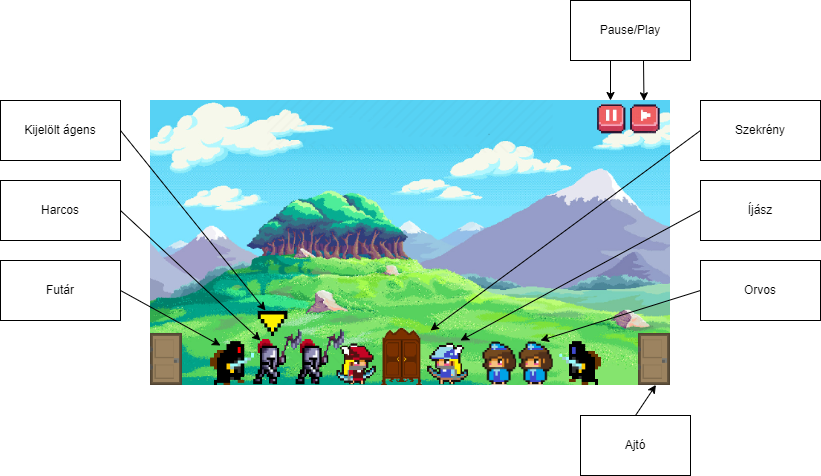
\includegraphics[width=\textwidth]{images/scene.png}
    \caption{szoba}
    \label{fig:scene}
\end{figure}
\newpage
\subsection{A szimulációban használt szobák bemutatása}

A szimulációban az ágensek szobákban mozoghatnak, a szobák pedig blokkokból épülnek fel.Egy blokk 50 x 50 nagyságú. Egy szoba 32  blokkból áll.16 blokk az ablak legalsó sorában illetve 16 blokk egy sorral efölött. Minden szobában 2 ajtó van kivéve az első és az utolsó szobát, ahol 1-1 zászló is van, a középső szobában van egy szekrény. Minden szobához tartozik egy egyedi háttérkép.
\newline
A szimuláció 5 szobából fog állni. Kezdetben az elsőtől a harmadik szobáig a 3-6 blokkig lenne a felállása a piros csapatoknak, a harmadiktól az ötödik szobáig a 11-14 blokkig lenne a felállása a kék csapatoknak. Egy blokkon egyszerre csak egy karakter állhat.

\subsection{A szimulációban használt objektumok jellegzetességei}

Ebben a részben az ajtó, zászló és a szekrény objektumok részletes leírása kerül bemutatásra.

Minden objektum mozgáskorlátozó hatással bír.
\newline
Az objektumok szélessége 1 blokk illetve magassága 2 blokk.
\newline
Ajtó működése:
\begin{itemize}
\item Az ajtók pozíciója fixen az első illetve a 16. blokkon van minden szobában.
\item A szélső blokkokon lévő ajtók használata után az ágens átkerül a következő szoba ellentétes oldalára, ami azt jelenti, hogyha a bal oldalán megy be akkor a jobb oldalon jön ki.
\item A teljes szimulációban nem lehet páratlan számú ajtó.
\item Minden ajtó fix pozícióra vezet át.
\item Ágensek egyesével tudják használni az ajtót.
\item Minden szobában maximum 2 ajtó lehet.
\item Különböző ajtók használata nem vezethet ugyanarra a blokkra.
\end{itemize}
Zászló működése:
\begin{itemize}
\item Az első szoba első blokkján illetve az utolsó szoba utolsó blokkján ajtó helyett a zászló van.
\item Zászlót felvenni csak ellenséges csapat ágense képes felvenni.
\item Minden csapatnak egyetlen zászlója van. Abban a szobában ahova egyetlen ajtó vezet és a saját egységei védik.
\item A felvétele után vége a szimulációnak.
\end{itemize}
Szekrény működése:
\begin{itemize}
\item A szobának középső 2 blokkján helyezkedik el.
\item A szekrény nem foglal helyet a térből.
\item Tárgyak tárolására funkcionál.
\item Csak a Futár osztállyal rendelkező ágens vehet ki tárgyakat a saját leltárába a szekrény leltárából.
\item A szekrény leltára félig kötszerrel,félig nyílvesszővel van feltöltve.
\item A szekrény 10 tárolóegységgel rendelkezik,fele-fele arányban feltöltve kötszerrel illetve nyílvesszővel.
\item Az alábbi ábrán megtekinthető(\ref{fig:map}.ábra)
\end{itemize}
\newpage

\begin{figure}[!ht]
	\centering
	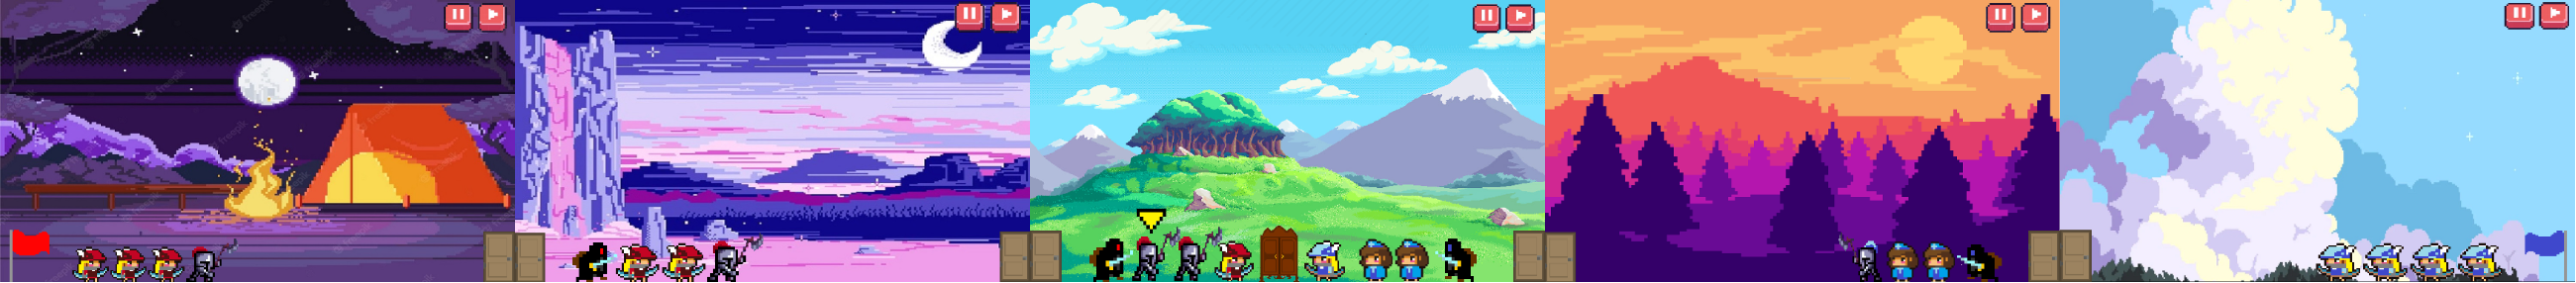
\includegraphics[width=\textwidth]{images/map.png}
    \caption{környezet}
    \label{fig:map}
\end{figure}
\section{Ágensek}

Ebben a fejezetben az ágens definiálása,tevékenységeiről és tulajdonságairól lesz szó.

Fontosabb tulajdonságai az önállóság,kommunikációs készség illetve alkalmazkodókészség. Önállóság alatt azt értjük, hogy saját maga dönti el, hogy adott helyzetben mit csinál emberi beavatkozás nélkül. Kommunikációs készség azt jelentené, hogy tudja érzékelni az őt körülvevő környezetet. Az Alkalmazkodókészség a változó környezet észlelésére optimális tevékenység kiválasztását teszi lehetővé.
\newline
Minden ágens 1 blokk szélességű és 2 blokk magas.
A szimuláció elején dől el melyik ágens melyik osztályba tartozik.
Egy osztályt több ágens is megkaphat.
Ágens csak azokat a tevékenységeket tudja végezni amelyet az osztálya megenged.
Minden ágensnek 4 tulajdonsága van ebből 1 osztálytól függően különbözik.

\subsection{Ágensek tevékenységei}

Mozgás:

\begin{itemize}
\item Ezt a tevékenység végrehajtó ágens megtudja változtatni a blokk pozícióját.
\item A ágensek 1 blokkonként tudják ezzel a tevékenységgel változtatni a helyzetüket.
\item Jobbra illetve balra tudnak mozogni az ágensek.
\item Mindig csak a két szomszédos blokkra tudnak átmenni.
\item Ezt a tevékenységet csak adott visszatöltési idő lejárta után lehet használni. 
\item Az idő mértéke az ágens osztályának statisztikáitól függ. 
\item A visszatöltési idő közben a karakter folytonosan mozog egyik blokkból a másikba.
\item Ha a szomszédos pozíció nem üres akkor nem lehet abba az irányba végezni ezt a tevékenységet.
\item Egyszerre több ágens is végezheti.
\item Csak támadás és guggolás mellett lehet egyidejűleg mozogni.
\end{itemize}

Ajtó kinyitása:

\begin{itemize}
\item Ezt a tevékenységet csak akkor tudja végrehajtani az ágens, ha az ajtóval szomszédos blokkon áll.
\item A kinyitást követően az ágens a következő szoba első blokkjára kerül.
\item Csapaton belül egyszerre csak egy ágens végezheti.
\item Nem lehet semmilyen más tevékenységet végezni ajtó kinyitás közben.
\item Ennek az akciónak végrehajtási ideje van ami az ágens osztályának statisztikáitól függ.
 
\end{itemize}

Helycsere:

\begin{itemize}
\item Csak ágensek között lehet használni.
\item Egy ágens akkor tud helyet cserélni, ha szomszédos blokkján van ágens.
\item Nem lehet más akciót végrehajtani helycsere közben.
\item Csapaton belül egyszerre csak 2 ágens cserélhet helyet és csak egymással.
\item Ennek a tevékenységnek visszatöltési ideje van ami függ az ágens osztályának statisztikáitól.
\end{itemize}

Szekrény kinyitása:

\begin{itemize}
\item Csak a Futár osztállyal rendelkező ágens tudja ezt a tevékenységet végrehajtani és csak akkor ha a szekrénnyel szomszédos blokkon áll.
\item Végrehajtáskor feltölti az ágens üres tárolóhelyét fele-fele arányban kötszerrel illetve nyílvesszővel. Ha csak egy üres tárolóhellyel rendelkezik az ágens akkor véletlenszerűen megkapja az egyiket.
\item Ennek a tevékenységnek van egy fix végrehajtási ideje. Amely az adott osztály statisztikájától függ.
\item A tevékenységgel párhuzamosan nem lehet végezni más tevékenységeket.
\item Egyszerre csak egy ágens végezheti ezt az akciót.
\end{itemize}

Támadás:

\begin{itemize}
\item Ezt a képességet használó ágens csökkenteni tudja más ágensek életerejét.
\item Ha egy ágens életereje 0 akkor nem lehet tovább támadni.
\item Ezt az akciót csak időközönként lehet használni.Az ágens osztályának statisztikájának nagyságától függ, hogy mekkora visszatöltési ideje van ennek az akciónak.
\item Ajtó kinyitása,Helycsere,Guggolás közben nem lehet támadni.
\item Mozgás tevékenység közben is lehet támadni. 
\item Egyszerre több ágens is végezheti ezt a tevékenységet.
\item Csak Íjász és Harcos osztályú ágensek tudják ezt a tevékenységet végezni.
\end{itemize}

Gyógyítás:

\begin{itemize}
  \item Ezt a képességet használó ágens vissza tudja tölteni más ágensek életerejét.
  \item Maximum életerő vagy 0 életerő esetén nem lehet gyógyítani.
  \item Gyógyítani csak az Orvos osztállyal rendelkező ágens tud.
  \item Csak akkor lehet végrehajtani, ha van kötszer az Orvos leltárában.
  \item Csak szövetséges ágenseket lehet gyógyítani.
  \item Fix időbe telik valakit gyógyítani. Eközben sem a gyógyító sem a gyógyuló nem végezhet más tevékenységeket. 
  \item Egyszerre több ágens is végezheti ezt a tevékenységet.
  \item Csak Orvos osztály végezheti ezt a tevékenységet.
\end{itemize}

Guggolás:

\begin{itemize}
  \item Az ágensek esetében van százalékos esély arra, hogy guggolás akciót használjon , abban a pillanatban amikor egy Íjász éppen támad ezzel elkerülve a sebzést.
  \item A guggolás hatása csak távharci támadás esetében érvényesül.
  \item Guggolás során karakterünk magassága megváltozik 1 blokkra.
  \item Guggolás közben csak mozogni lehet más tevékenységet nem lehet végezni.
  \item Ennek az akciónak van visszatöltési ideje.Az ágens gyorsaságától függ mennyi a visszatöltési idő.
  \item Egyszerre több ágens is végezheti ezt az akciót.
\end{itemize}

Átadás:

\begin{itemize}
  \item Ezt a képességet használó ágens tárgyakat tud átadni más ágenseknek.
  \item Fix végrehajtási időbe telik ennek a tevékenységnek az elvégzése.
  \item Csak a futár osztállyal rendelkező ágens képes tárgyakat átadni.
  \item Átadás közben csak az átadó nem tud végezni más cselekvést. Akinek átadnak csak mozogni nem tud a végrehajtási időig.
  \item Csak akkor lehet végezni ha a szomszédos blokkon szövetséges ágens áll.
  \item Egyszerre több ágens is végezheti.
  \item Ellenséges ágenseknek nem lehet átadni tárgyakat.
\end{itemize}

\subsection{Ágens tulajdonságok}

Ezek a tulajdonságok minden szimuláció kezdetén az osztályok statisztikái alapján értékelődnek ki.
\newline
Életerő:
\begin{itemize}
\item Minden ágens életerejének van felső határa, aminek értéke az osztályának vitalitási értékétől függ.
\item Minden ágens kezdeti életereje egyenlő az életereje felső határával. 
\item Típusa pozitív egész, amely 0 érték alá nem mehet.
\item Ha az ágens életerőt vesztett akkor a felső határig lehet növelni gyógyítási értékkel.
\item Ha valamelyik ágens életereje eléri az alsó határt azaz 0 értéket akkor az az ágens meghal.
\item Az ágens halál után megszűnik.
\item Az életerő csak akkor csökken ha az ágenst sebzik.
\item Az életerő egy csíkként jelenik meg az ágensek felett amelynek közepében van az aktuális értéke feltüntetve.
\end{itemize}

\noindent Védelem:

\begin{itemize}
\item Minden ágensnek van egy kezdeti védelme aminek értéke minden osztályán esetében más statisztikától függ.
\item A szimuláció kezdete után ez egy fix érték, nem fog változni a szimuláció végéig.
\item Típusa pozitív egész.
\item Ha az ágens sebzést kapna ezt az értéket vonjuk le először a támadásból majd a megmaradt sebzéspontok az ágens életerejéből vonódnak le.
\end{itemize}

\newpage

\noindent Várakozási idő:

\begin{itemize}
  \item Minden ágensnek van egy kezdeti gyorsasága aminek értéke minden osztály esetében más statisztikától függ.
  \item Típusa pozitív egész.
  \item A gyorsaság befolyásolja az ágens várakozási idejét.
  \item Minél nagyobb ez az érték annál kisebb a várakozási idő.
  \item Csak azokat a tevékenységeket befolyásolja amelyeknél van várakozási idő.
  \item A szimuláció kezdete után ez egy fix érték, nem fog változni a szimuláció végéig.
\end{itemize}

\noindent Végrehajtási idő:

\begin{itemize}
\item Minden ágensnek megvan szabva osztály statisztikák alapján, hogy mekkora a tevékenységek végrehajtási ideje.
\item Csak olyan tevékenységeknél értékelődik ki amelyeknek van végrehajtási ideje.
\item Típusa pozitív egész.
\item Minél nagyobb ez az érték annál kevesebb idő a vérhajtása a tevékenységeknek. 
\item A szimuláció kezdete után ez egy fix érték, nem fog változni a szimuláció végéig.
\end{itemize}

\noindent Támadó érték:
\begin{itemize}
\item Csak olyan ágens osztályok rendelkeznek támadó értékkel amelyek végre tudják hajtani a támadás tevékenységet.
\item Típusa pozitív egész.
\item Osztályok esetében különböző statisztikák alapján értékelődik ki.
\item Ez szabja meg, hogy a megtámadott ágensnek az életereje mekkora értékkel fog csökkenni.  
\item A szimuláció kezdete után ez egy fix érték, nem fog változni a szimuláció végéig.
\end{itemize}

\noindent Gyógyítási érték:
\begin{itemize}
\item Csak azaz ágens rendelkezi ezzel az értékkel amely képes végrehajtani a gyógyítás tevékenységet.
\item Típusa pozitív egész.
\item Csak az Intelligencia statisztika alapján értékelődik ki.
\item Ez szabja meg, hogy a gyógyított ágens életereje mennyivel fog a felső határig növekedni.
\item A szimuláció kezdete után ez egy fix érték, nem fog változni a szimuláció végéig.
\end{itemize}

\section{Osztályok}

Négy fajta osztály van:
\begin{itemize}
\item Harcos,Íjász,Orvos,Futár.
\end{itemize}

\subsection{Harcos}
\begin{itemize}
 \item A harcos végre tudja hajtani a támadást,mozgást,ajtó kinyitást,guggolást.
 \item Helycserét nem tud kezdeményezni de ha egy másik ágens rajta akarja végrehajtani ezeket a tevékenységeket az lehetséges.
 \item A harcos osztállyal rendelkező ágensek támadásának hatótávolsága a szomszédos blokkokig terjed.
 \item Életerejének felső határát a vitalitás statisztika növeli.
 \item Minden egyes pont a vitalitáson 2-el növeli a maximális életerő értékét.
 \item Támadó értéket az erő statisztika növeli.
 \item Minden egyes pont az erőn 1-el növeli a támadó értéket.
 \item Védelmet az ügyesség statisztika növeli.
 \item Minden egyes pont az ügyességen 1-el növeli a védelmet.
 \item A várakozási időt a gyorsaság statisztika befolyásolja.
 \item Minden egyes pont a gyorsaságon 0.1 másodperccel csökkenti a várakozási időt.
 \item A végrehajtási időt az intelligencia statisztika befolyásolja.
 \item Minden egyes pont a intelligencián 0.1 másodperccel csökkenti a végrehajtási időt.
 \item Gyógyítási értéke ennek az osztálynak nincs.
 \item Ennek az osztálynak nincs leltára.
 \item Csak közelharci fegyvereket használhatnak.
\end{itemize}

\subsection{Íjász}
\begin{itemize}
\item Az Íjász végre tudja hajtani a támadást,mozgást,ajtó kinyitást,guggolást.
\item Helycserét illetve Átadást nem tud kezdeményezni de ha egy másik ágens rajta akarja végrehajtani ezeket a tevékenységeket az lehetséges.
\item Az Íjász osztállyal rendelkező ágensek támadásának hatótávolsága a helyzetétől kezdve egy fix blokknyi távolság lehet.
\item Életerejének felső határát a vitalitás statisztika növeli.
\item Minden egyes pont a vitalitáson 2-el növeli a maximális életerő értékét.
\item Támadó értéket az ügyesség statisztika növeli.
\item Minden egyes pont az ügyességen 2-el növeli a támadó értéket.
\item Védelmet az erő statisztika növeli.
\item Minden egyes pont az erőn 1-el növeli a védelmet.
\item A várakozási időt a gyorsaság statisztika befolyásolja.
\item Minden egyes pont a gyorsaságon 0.1 másodperccel csökkenti a várakozási időt.
\item A végrehajtási időt az intelligencia statisztika befolyásolja.
\item Minden egyes pont a intelligencián 0.1 másodperccel csökkenti a végrehajtási időt.
\item Gyógyítási értéke ennek az osztálynak nincs.
\item Van leltára.
\item Csak távharci fegyvereket képesek használni.
\end{itemize}

\subsection{Orvos}
\begin{itemize}
\item Az Orvos nem tudja végrehajtani a támadást,szekrény kinyitását,átadást.
\item Átadást nem tud kezdeményezni de ha egy másik ágens rajta akarja végrehajtani ezt a tevékenységet az lehetséges.
\item Csak szomszédos blokkon lévő ágensek esetében tudnak gyógyítani.
\item Másodpercenként automatikusan gyógyítja saját magát 1 életerőponttal.
\item Életerejének felső határát a vitalitás statisztika növeli.
\item Minden egyes pont a vitalitáson 1-el növeli a maximális életerő értékét.
\item Gyógyítási értéket az intelligencia statisztika növeli.
\item Minden egyes pont az intelligencián 1-el növeli a gyógyítási értéket.
\item Védelmet az erő statisztika növeli.
\item Minden egyes pont az erőn 2-el növeli a védelmet.
\item A várakozási időt a gyorsaság statisztika befolyásolja.
\item Minden egyes pont a gyorsaságon 0.1 másodperccel csökkenti a várakozási időt.
\item A végrehajtási időt az ügyesség statisztika befolyásolja.
\item Minden egyes pont a ügyességen 0.1 másodperccel csökkenti a végrehajtási időt.
\item Támadó értéke ennek az osztálynak nincs.
\item Van leltára.
\item Ez az osztály nem használ fegyvereket.
\end{itemize}

\subsection{Futár}
\begin{itemize}
\item A Futár nem tudja végrehajtani a támadást és a gyógyítást.
\item Csak szomszédos blokkon lévő ágensek esetében tudnak átadni.
\item Életerejének felső határát a vitalitás statisztika növeli.
\item Minden egyes pont a vitalitáson 3-el növeli a maximális életerő értékét.
\item Védelmet az erő statisztika növeli.
\item Minden egyes pont az erőn 1-el növeli a védelmet.
\item A várakozási időt a gyorsaság illetve az intelligencia statisztika befolyásolja.
\item Minden egyes pont a gyorsaságon és az intelligencián 0.1 másodperccel csökkenti a várakozási időt.
\item A végrehajtási időt az ügyesség statisztika befolyásolja.
\item Minden egyes pont a ügyességen 0.2 másodperccel csökkenti a végrehajtási időt.
\item Ennek az osztálynak nincs gyógyítási illetve támadó értéke.
\item Van leltára.
\item Ez az osztály nem használ fegyvereket.
\end{itemize}

\subsection{Kezdeti statisztikák}

Minden ágensre a statisztikák értéke véletlenszerűen fog legenerálódni a szimuláció kezdetekor.

\begin{table}[!ht]
\centering
\caption{Kezdeti statisztikák intervalluma}
\label{tab:table1}
\begin{tabular}{|l|c|c|c|c|}
\hline
 & Harcos & Íjász & Orvos & Futár \\
\hline
Erő & 1-5 & 1-3 & 1-4 & 1-2  \\
\hline
Intelligencia & 1-5 & 1-3 & 1-4 & 1-2  \\
\hline
Ügyesség & 1-5 & 1-3 & 1-4 & 1-2 \\
\hline
Vitalitás & 1-5 & 1-3 & 1-4 & 1-2 \\
\hline
Gyorsaság & 1-5 & 1-3 & 1-4 &1-2 \\
\hline
\end{tabular}
\end{table}

\section{A környezet észlelése}

Az ágensek folyamatosan egy irányba haladnak.
\newline
Az objektumok észlelése:
\begin{itemize}
\item A szimuláció elején megkapják az ágensek az ellenség zászlójának helyzetét.
\item A szimuláció során arra törekednek, hogy minél közelebb legyenek az ellenséges zászlóhoz.
\item A csapatok nem ismerik a szövetséges zászló helyzetét.
\item Ajtók jelenlétét csak szomszédos blokkokon vizsgálják az ágensek.
\item A Szekrényt csak a Futár osztállyal rendelkező ágensek látják és a szimuláció kezdetétől tudják a helyzetét, csak akkor indulnak el a szekrény irányába ha hátizsákjuk teljesen kifogyott.
\end{itemize}

\noindent Ágensek egymás közti észlelésének szabályrendszere:

\begin{itemize}
	\item A szimuláció kezdetétől tudják az ágensek, hogy ki ellenség, ki szövetséges amit a csapat változóból tudnak.
	\item Minden ágens aki egy csapatba tartozik megkapja ugyanazt a változót ugyanazzal az értékkel.
	\item Az ágensek nem mozdulnak kezdeti helyükről amíg nem észlelnek ellenséges ágenst.
	\item Minden ágens észlelése és az ehhez szorosan hozzátartozó tevékenységek végrehajtása az ágens osztályától függ. 
\end{itemize}

\subsection{Harcos ágens észlelése}

\begin{itemize}
  \item Megvizsgálja hogy a közvetlen közelében van-e ellenség ha nincs akkor addig megy amíg nem lesz a közelében ellenfél.
  \item Ha hatótávolságba ér akkor támad a támadást addig végzi amíg az adott ellenfél meg nem hal vagy nem kezd el kimenni a támadás hatósugarából.
  \item Harcosok közelharci támadás hatóköréből nem tudnak menekülni viszont minden közelharci támadásra van esélyük a kivédésre.
  \item Ha az ellensége akivel harcol meghal elindul a következő legközelebbi ellenség irányába és megtámadja.
\end{itemize}

\subsection{Íjász ágens észlelése}

\begin{itemize}
  \item Az Íjásznak a harc kezdetekor el kell döntenie, hogy az ellenség csapatából kit fog támadni, csak azokat az ellenfeleket képes támadni akik a hatótávjában vannak prioritás alapján.
  \item Eldöntés után addig támadja ezt a ágenst amíg az meg nem hal vagy ki nem fogy a Nyílvesszőkből.
  \item Ha meghal az ágens akit támadott akkor a prioritásban következő ellenséget támadja.
  \item Minden egyes támadás után az Íjász leltárából eltűnik egy nyílvessző.
  \item Ha az Íjász ágensnek elfogy a leltárából a nyílvessző akkor üzen a Futárnak, hogy szüksége van a számára megfelelő tárgyakra.
  \item Ha elfogyott a nyílvessző és nem kap utánpótlást akkor addig nem támad amíg nem lesz a leltárában nyílvessző.
  \item Ez az osztály mindig tart egy fix távolságot a legközelebbi ellenféltől.
\end{itemize}

Az Íjász támadási prioritása:

\begin{itemize}
  \item Gyógyító
  \item Futár
  \item Íjász
  \item Harcos
\end{itemize}

\subsection{Orvos ágens észlelése}

\begin{itemize}
  \item Az Orvos folyamatosan a szövetségesei életerejét vizsgálja,ha egy ágens életereje x\% alá esik akkor üzen az Orvos ágensnek, hogy gyógyításra van szüksége.
  \item Ennek hatására az Orvos odamegy az üzenet küldő ágens közvetlen közelében és elkezdi őt gyógyítani.
  \item A gyógyítás fix időn belül megtörténik és eltűnik egy kötszer az Orvos leltárából.
  \item A prioritás mindig annál a ágensnél van aki a legrégebben küldte az üzenetet.
  \item Csak az Orvos osztállyal lehet gyógyítani.
\end{itemize}

\subsection{Futár ágens észlelése}

\begin{itemize}
  \item A Futár folyamatosan a szövetséges Orvos illetve Íjász leltárát vizsgálja.
  \item Ha az Orvos illetve a Íjász ágensnek elfogy a leltárából a kötszer vagy nyílvessző akkor üzen a Futárnak, hogy szüksége van a számára megfelelő tárgyakra.
  \item Erre az üzenetre reagálva a Futár feltölti az üzenetet küldő ágens hátizsákját azzal a tárggyal amit kért.
  \item Mindkét osztály csak akkor küld üzenetet ha teljesen kifogytak. Ennek oka az, hogy leltárukban csak ez az egyfajta tárgy lehet és fölösleges minden egyes elhasznált tárgyat pótolni.
  \item A prioritás mindig annál a ágensnél van aki a legrégebben küldte az üzenetet ellenkező esetben fennáll az a lehetőség sok üzenetküldés esetén, hogy valaki sose kap választ.
  \item Futárok egymás között tudnak átadni tárgyakat.
  \item A harc fázis végén feltöltődik a futár leltára félig nyílvesszővel félig kötszerrel.
  \item Csak a Futár osztállyal lehet tárgyakat átadni.
\end{itemize}

\section{Az ágens csapatok osztályainak kiosztására vonatkozó szabályrendszer}

\begin{itemize}
	\item Futár osztályból minden csapatban egynek kell. lennie.
	\item Az Orvos osztályból legfeljebb csak 2 lehet minden csapatban.
	\item Harcosokra és Íjászokra nincs kikötés.
\end{itemize}

\section{Harc}

\subsection{Harc fázis}

A harc az egy külön fázis, amely akkor kezdődik amikor a csapat minden tagja észleli az ellenfél csapatát és szövetségeseit.A harci fázisnak akkor van vége hogyha az egymással szemben álló valamelyik csapatból az összes tag meghal. A fázis elején dől el, hogy a ágensek kikre tekintenek szövetségesként és kikre ellenfélként.

\subsection{Sebzés kalkulálása}

Sikeres támadás esetén a sebzés mértéke 0 ha a harci hatások valamelyike érvényesül vagy időben lett használva a guggolás. Más esetben a sebzés mértékét befolyásolja az adott ágens védelme, ez az érték levonódik a sebzés értékéből majd az eredményt levonjuk a védekező ágens életerejéből.

Védekezés:
\begin{itemize}
\item Ez a hatás százalékos eséllyel aktiválódik minden egyes ellenfél által bevitt sikeres támadás esetén.
\item Ez egy állandó hatás.Csak a Harcos rendelkezik ezzel a hatással.
\end{itemize}

Kitérés:
\begin{itemize}
\item Ez a hatás \%-os eséllyel aktiválódik minden egyes ellenfél által bevitt sikeres közelharci támadás esetén.
\item Ez egy állandó hatás.Csak az Íjász rendelkezik ezzel a hatással.
\end{itemize}

\newpage

\section{Tárgyak}

\begin{table}[!ht]
\centering
\caption{Tárgyak}
\label{tab:table2}
\begin{tabular}{|l|c|c|c|c|}
\hline
 & Osztály &Típus & Támadás & Védelem  \\
\hline
Kard & Harcos & Közelharc & 1-5 & 0 \\
\hline
Íj & Íjász & Távharc & 1-5 & 0  \\
\hline
Mellvért & Harcos & Közelharc & 0 & 3   \\
\hline
Mellény & Íjász & Közelharc & 0 & 1   \\
\hline
Köpeny & Orvos & Közelharc & 0 & 2    \\
\hline
Ruha & Futár & Közelharc & 0 & 2    \\
\hline
\end{tabular}
\end{table}

Speciális tárgyak:
\begin{itemize}
  \item Kötszer:Csak az orvos képes használni.Fogyóeszköz. 3 életerőt lehet vele gyógyítani.
  \item Nyílvessző:Csak Íjász képes használni.Fogyóeszköz.Ha elfogy az egység nem tud támadni.
  \item Pajzs:Csak a Harcos használhatja. 10\% védekezési esélyt nyújt de csak közelharcban.
\end{itemize}
    
\section{Hátizsák}

\begin{itemize}
  \item A hátizsák egy megjelenő menü amit a TAB billentyűvel lehet megnyitni 1 páncél,1 fegyver és 10 tárolóhelyből áll.
  \item Teljesen megegyező és különböző tárgyak külön-külön helyen fognak tárolódni.
  \item Az ágensek közötti tárgy átadásnál a tárgy az adó ágens leltárából törlődik a vevő ágensnél megjelenik.
  \item Ha egy tárgyat kihúzunk a hátizsák menüjén kívülre, akkor a tárgy törlődik.
  \item Más szövetséges ágensek hátizsákját csak a Futár osztály láthatja olyan ágenseknek nem látja akiket ellenségként észlel.
  \item Ha egy ágens meghal a teljes hátizsákja törlődik.
  
\end{itemize}

\subsection{Osztályokra specializált szabályok}
\begin{itemize}
  \item Az Íjász osztály teljes leltára a szimuláció kezdetekor  nyílvesszővel van feltöltve.
  \item Az Íjász leltárában csak nyílvesszők lehetnek.
  \item Az Orvos osztály teljes leltára a szimuláció kezdetekor kötszerrel van feltöltve.
  \item Az Orvos leltárában csak kötszerek lehetnek.
  \item A Futár leltára a szimuláció kezdetén félig nyílvesszővel, félig kötszerrel van feltöltve.
  \item Csak a Futár osztály képes ágensek között tárgyakat átadni.
  \item A Harcos osztály hátizsákja üres.
  
\end{itemize}












